\section{自然语言处理相关技术}
自然语言处理(NLP)的定义可以简单概括对人类语言进行自动化、智能化分析以及学会人类表达的一系列计算机技术,是一门包含着计算机科学、时间序列分析以及语言学的交叉学科,这些学科既有区别又相互交叉。

1936年A.M.Turing发明了举世闻名的“图灵机”,使数学中的逻辑符号和真实世界之间建立了联系,为后来计算机的蓬勃发展提供了坚实的理论基础。20世纪50年代,在图灵机的计算模型的基础上,自动机理论被提出,是现代计算机科学发展的基础\cite{自然语言处理的历史与现状}。后来Kleene又在自动机理论模型之基础上提出了正则表达式和有限自动机。1956年,Chomsky提出了上下文无关的语法的理论,同年人工智能被发明后,被迅速应用到自然语言处理领域之中。上下文无关语法的提出使得该领域的研究分为了基于推理规则的符号派和基于概率论的随机派\cite{宋一凡2019自然语言处理的发展历史与现状},在之后很多年里分别高速发展。70年代语音识别算法研制成功,隐马尔科夫模型(Hidden Markov Model,HMM)提出并得到了广泛应用\cite{自然语言处理的历史与现状}。

近年来,随着深度学习的飞速发展,自然语言处理领域也取得了诸多重要突破。RonanCollobert等\cite{Natural_language_processing_(almost)_from_scratch}于2011年的研究提出了一个简单的深度学习框架,在许多NLP经典任务中取得了前所未有的性能,如实体命名识别、语义标注和词性标注等。之后,研究人员提出了大量基于复杂深度学习的算法,用于解决有难度的NLP任务。2013年,Mikolv\cite{skipgram}提出了当前NLP领域最重要的模型之一Skip-gram,该模型以出色的性能表现将单词转化为高维向量,为后续如雨后春笋般涌现的自然语言处理模型奠定了基础。

本章后续内容以词嵌入方法、循环神经网络等主流自然语言处理模型为基础,探讨其在文件系统优化,尤其是数据迁移策略中“冷”、“热”文件分类问题的应用。

\subsection{词嵌入}

%\href{https://www.linkresearcher.com/careers/6c7a15b5-236a-40f3-879f-af2ac06c2557}{NLP综述博客}
%\href{https://blog.csdn.net/mawenqi0729/article/details/80698350}{词嵌入博客}

众所周知,在自然语言处理任务中,第一步工作就是用计算机能够理解的方式表示和描述单词,也就是将其用向量表示。通常有两大类表征方式:离散型表示(one-hot)和分布型表示(distributed representation)。

所谓离散型表示是指,在给定词汇表$V$的条件下,每一个单词被表示为一个维度为$|V|$的向量,该词汇表中任意一个单词,唯一地分配一个维度为1,其余维度均为0。例如单词file在词汇表中第二个出现,则其离散型向量表示为:$v_{file} = [0,1,0,\dots,0]$。这种表示方式相当于为每个单词分配了一个唯一的ID。当词汇表较大时,词嵌入的维度将会非常高,并且无法表达词与词之间的关系。

单词的分布式表示基于语义学中的分布式假设(Distributional Hypothesis)\cite{distributional_hypothesis}:
在相似的上下文中出现的单词通常具有相似的含义。例如单词water和coffee常与drink搭配,因此water与coffee具备一定的的相似性。分布式表示的目的就是将单词转化为稠密的向量(与离散型的one-hot向量相对),将人类自然语言中的单词之间的相似性和逻辑关联转化为向量空间的数学关系来处理(例如使用二范数表达单词的相似度)。见图\ref{fig:t_sne}所示例子,Li等人\cite{visualizing}采用t-SNE方法对60维的词嵌入进行降维处理,结果显示,含义相近的单词在向量空间内“距离”也比较接近。
\begin{figure}[htp]
\centering
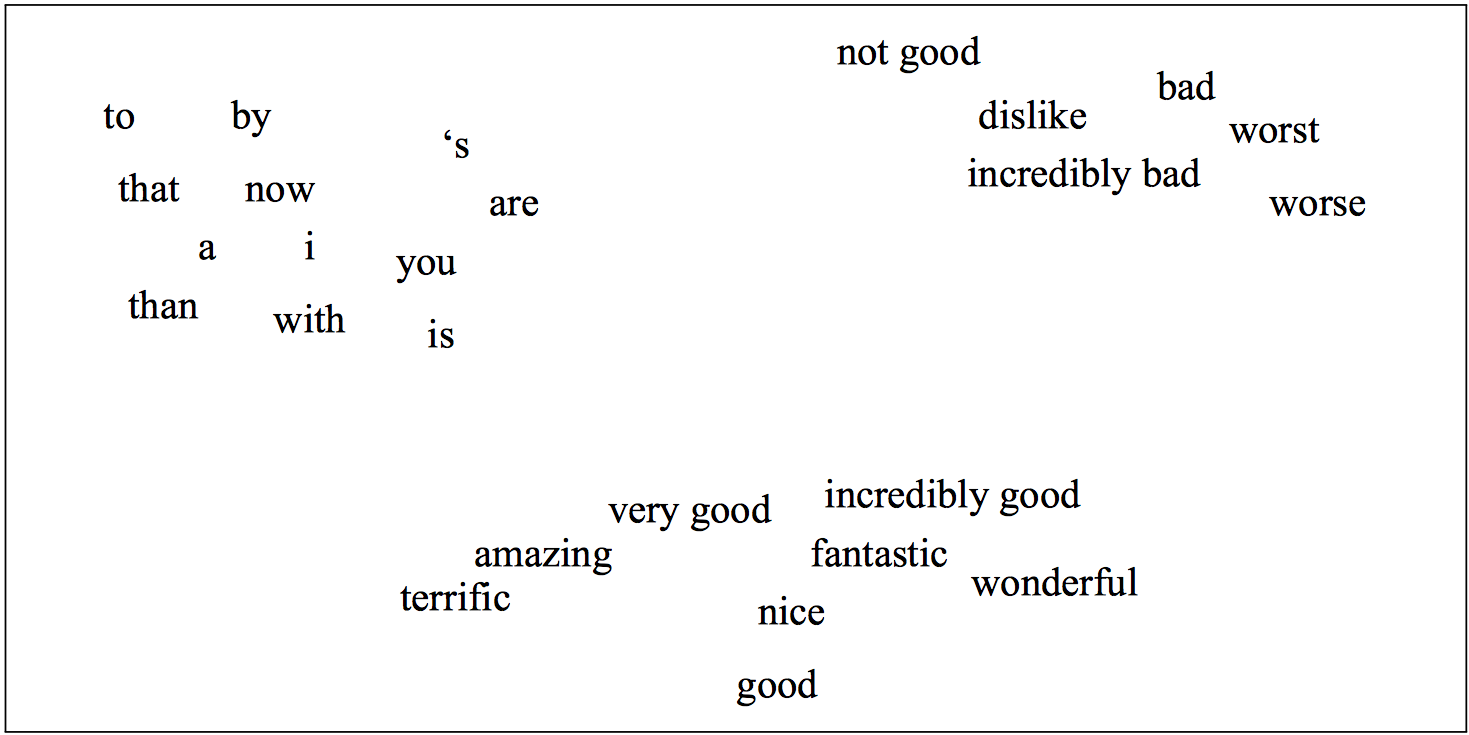
\includegraphics[width=\textwidth]{t_sne}
\caption{词向量降维后的可视化}
\label{fig:t_sne}
\end{figure}
%{\color{red}词嵌入降维图}\linkout{nlp_book}{107}

%{\color{red}词嵌入相关文献}\linkout{nlp_book}{128}

为实现这种从自然语言到向量空间的映射,自然语言处理发展历史上出现了许多理论和方法,例如Deerwester于1988年提出的潜在语义索引(Latent Semantic Indexing)方法\cite{LSI},以及该作者后续应用奇异值分解(SVD)对共现矩阵降维而实现的潜在语义分析方法(latent semantic analysis)\cite{LSA},在此后多年里被广泛应用于多种NLP任务,如认知模型\cite{cognitive_model},拼写检查\cite{spell_checking},写作评分\cite{essay_grading}等等。

随着近年来深度学习的发展,基于神经网络的自然语言模型开始流行,Bengio分别在2003年\cite{bengio2003}和2006年\cite{bengio2006}发表的成果表明,神经网络语言模型能在单词预测任务中出色地担任词嵌入转换的角色。

2013年,Mikolov提出了著名的连续词袋(CBOW)和Skip-gram模型\cite{skipgram},可以说这两种词嵌入模型的发明引发了NLP领域的深刻变革,至今为止这两种模型组成的Word2Vec方法仍被广泛使用于学术界和工业界。

Word2Vec是以无监督的方式从海量文本语料库中学习语义知识的一种模型,已被广泛应用在自然语言处理中。那么其实现的原理是怎样的?Word2Vec的根本原理是用词向量的方式表征词与词之间的语义信息,即通过将单词映射到一个高维空间来表征相近词之间的关联。这里的映射就是词嵌入。

Word2vec中实现的词向量训练方式有两种,Skip Gram和CBOW(constinuous bags of words),其中Skip Gram根据目标单词对上下文可能出现的单词进行预测,CBOW则相反,它通过上下文预测目标单词,最后使用模型的部分参数作为词向量。接下来,本文以Skip-gram算法为例进行原理介绍。

假设语料库中单词总数为$T$,其词汇表$\mathcal{V}$中的词汇数量为$W$。
%其中任意一个词可用其在词汇表中的序号表示:$w \in \{1,\dots,W\}$。
那么该语料库可表示为一个由$T$个词向量组成的序列:$\mathbf{w}_1, \mathbf{w}_2, \dots, \mathbf{w}_T$。Skip-gram模型的目标就是建立一个从该词汇表中所有文件名和目录名到$d$维向量空间的映射$model:\mathcal{V} \rightarrow \mathbb{R}^d$,使以下对数极大似然函数达到最大:
\begin{equation}
    \label{eq:origin_object}
    \frac{1}{T}\sum_{t=1}^T \sum_{c \in \mathcal{C}_t} \log p(\mathbf{w}_c | \mathbf{w}_t),
\end{equation}
取负号得到损失函数:
\begin{equation}
    L(\theta)= -\frac{1}{T}\sum_{t=1}^T \sum_{c \in \mathcal{C}_t} \log p(\mathbf{w}_c | \mathbf{w}_t),
\end{equation}

其中,$\mathcal{C}_t$表示某中心词$\mathbf{w}_t$的上下文中出现过的词的集合。对于任意样本$(\mathbf{\mathbf{w}}_t,\mathbf{\mathbf{w}}_c)$,我们可用归一化函数softmax来定义单词$\mathbf{w}_c$在中心词$\mathbf{\mathbf{w}}_t$的上下文中出现的条件概率:
\begin{equation}
    \label{eq:softmax}
    p(\mathbf{w}_c | \mathbf{w}_t)=\frac{ e^{ \mathbf{w}_t^{\top} \mathbf{w}_c} }{ \sum_{j=1}^W e^{\mathbf{w}_t^{\top} \mathbf{w}_j}} 
\end{equation}

Skip-gram模型是一个三层神经网络,输入为词汇表中单词的初始向量,即$W$维的one-hot编码。隐层由$d$个神经元组成,没有激活函数,只有权值。训练收敛后隐层的$W\times d$的权值矩阵就是词汇表内所有词向量的集合。输出层为上文所述的softmax函数,最终结果是一个$W$维的向量,每个分量表示对应的单词与输入词存在上下文关系的概率。

当语料库规模较大,词汇表内单词较多时,采用softmax函数的计算复杂度过高。一种优化方式是使用层次化softmax(Hierarchical softmax)\cite{Hierarchical_softmax}。另一种计算复杂度更低,且同样能保证对原有softmax层拟合精度的优化方式是负采样(Negative sampling)。该方法将原来的预测上下文的问题转化为一系列独立的二分类问题,即,在选定中心词后,对词汇表中其他单词依次判定是否在中心词附近出现。


对任意中心词$\mathbf{w}_t$,用交叉熵损失函数(Cross-entropy Loss)代替原来的损失函数
\begin{equation}
    \label{eq:loss_of_t}
    L_t(\theta) = -\left( 
        \sum_{c \in \mathcal{C}_t} \log(p(\mathbf{w}_c | \mathbf{w}_t))+\sum_{c \in \mathcal{N}_t} \log(1-p(\mathbf{w}_c | \mathbf{w}_t)) 
    \right)
\end{equation}
其中$\mathcal{C}_t$表示中心词$w_t$的上下文单词集合(正样本),$\mathcal{N}_t$表示词汇表中,与$w_t$不存在上下文关系的单词(负样本)中随机抽取的若干噪声词。

由于任意单词与中心词是否上下文被视为独立事件,可用sigmoid函数拟合条件概率
\begin{equation}
    p(\mathbf{w}_c | \mathbf{w}_t) = \frac{1}{1+e^{-\mathbf{w}_t^{\top} \mathbf{w}_c}} = \sigma(\mathbf{w}_t^{\top} \mathbf{w}_c)
\end{equation}

代入\ref{eq:loss_of_t}并按$t$累加求平均,得到最终的损失函数:
\begin{equation}
    L(\theta) = -\frac{1}{T}\sum_{t=1}^{T} \left[
        \sum_{c \in \mathcal{C}_t} \log(\sigma(\mathbf{w}_t^{\top} \mathbf{w}_c)) + \sum_{c \in \mathcal{N}_t} \log(\sigma(-\mathbf{w}_t^{\top} \mathbf{w}_c))
    \right]
\end{equation}

在Word2Vec中,无论是连续词袋模型还是Skip-gram,都将单词作为基本单元,为每一个单词生成一个向量。这种映射方式使得单词内部的形态和构造特征被忽略。与此同时,Word2Vec对陌生或低频单词的嵌入支持不好,当遇到语料库之外的单词时效果不好。

FastText的出现弥补了Word2Vec这些缺点。该模型采用字符级别的n-gram来表示单词,即,每个单词都是由子词(subword)构成,这些子词被以n-gram的形式存储和使用。基于字词建模后,完整单词的向量由其包含的字词向量相加得来。


\subsection{循环神经网络概述}
%简述RNN发展情况

循环神经网络最核心的功能是处理和预测序列类型的数据。在全连接神经网络或卷积神经网络模型中,网络的结构通常由输入层、隐藏层以及输出层构成,输入的样本数据相互独立,没有前后联系。而循环神经网络的功能结构有着本质区别,隐藏层之间的节点是有连接的,隐藏层的输入不仅仅由输入层的输出决定,还包括前一时刻隐藏层输出的隐状态,临近的样本数据包含的数据得以保持,因此具备了处理序列数据的能力。

\begin{figure}[htp]
\centering
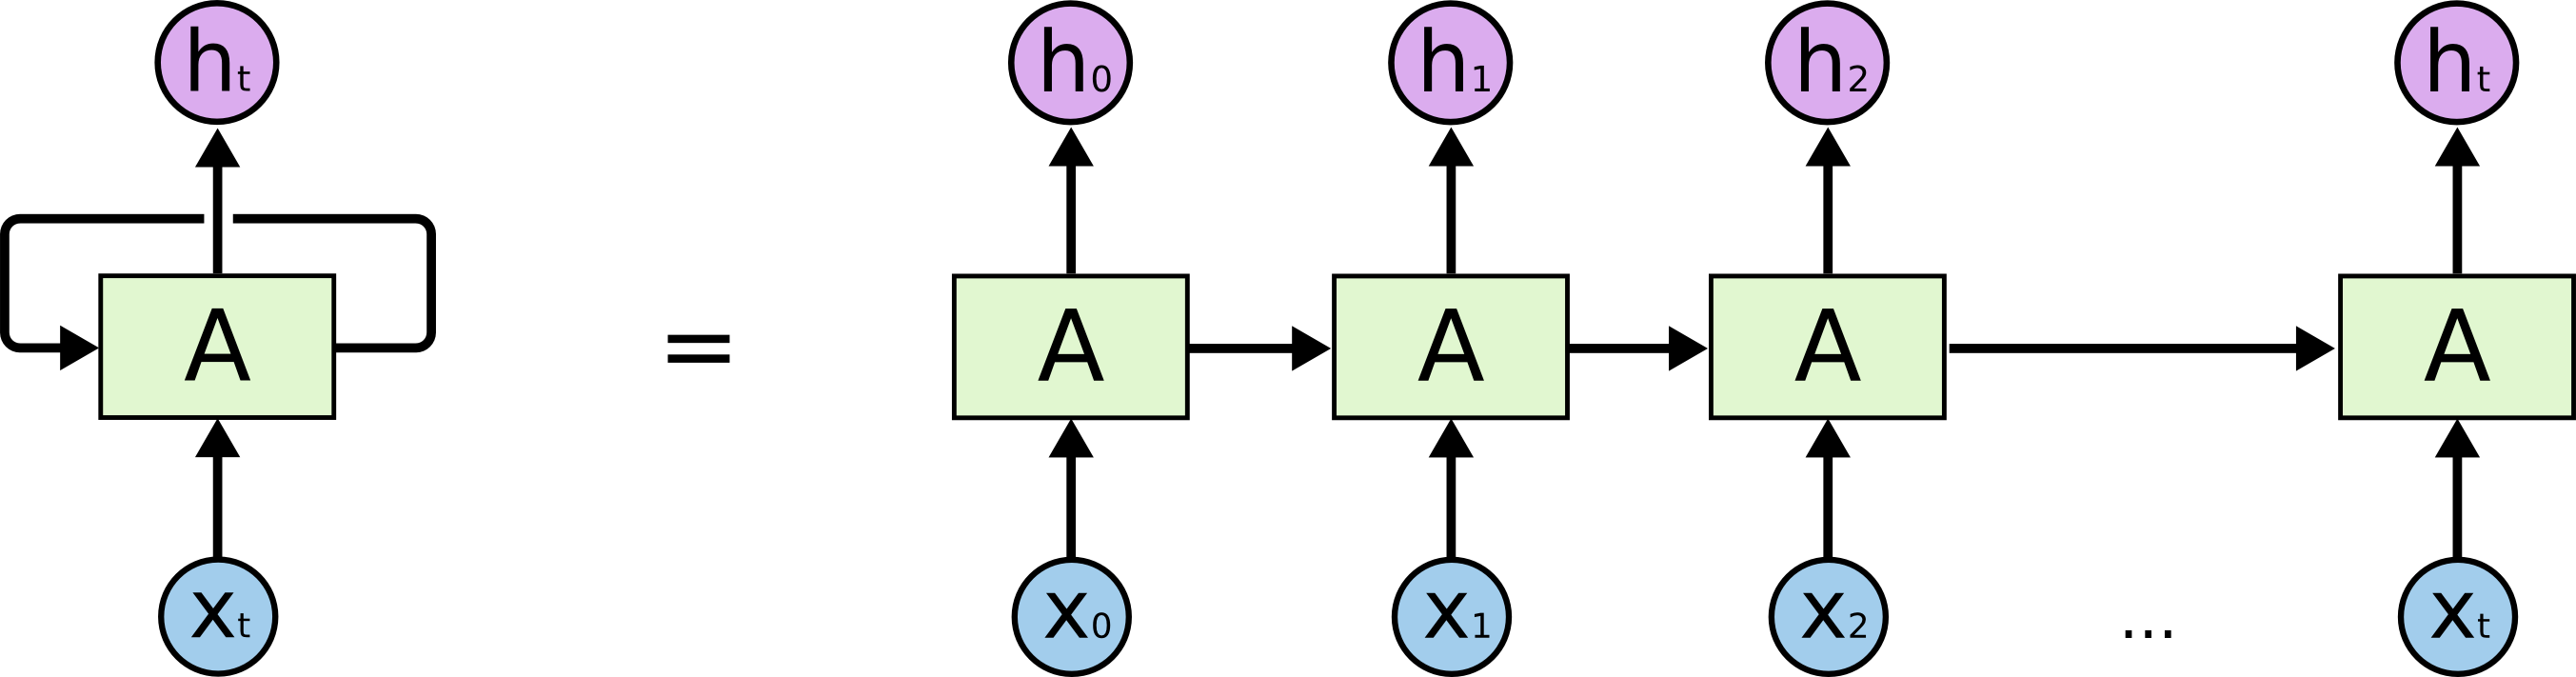
\includegraphics[width=\textwidth]{rnn_1}
\caption{RNN展开后的结构}
\label{fig:rnn_1}
\end{figure}
循环神经网络中区别于全连接或卷积神经网络的一个重要的概念就是时刻,输入数据以时间为标记。循环神经网络展开后如图\ref{fig:rnn_1}显示,除了来自输入层的样本数据$X_t$,还有一部分由前一时刻隐状态的计算结果提供。在每一个时刻,循环神经网络的运算单元会读取t时刻的输入$X_t$,并输出一个隐状态值$H_t$,同时将该隐状态传递到下一步。循环神经网络理论上可看作是一系列数据通过同一网络结构循环计算的结果。RNN根据输入输出对应关系可分为如下几类:

\begin{figure}[htp]
\centering
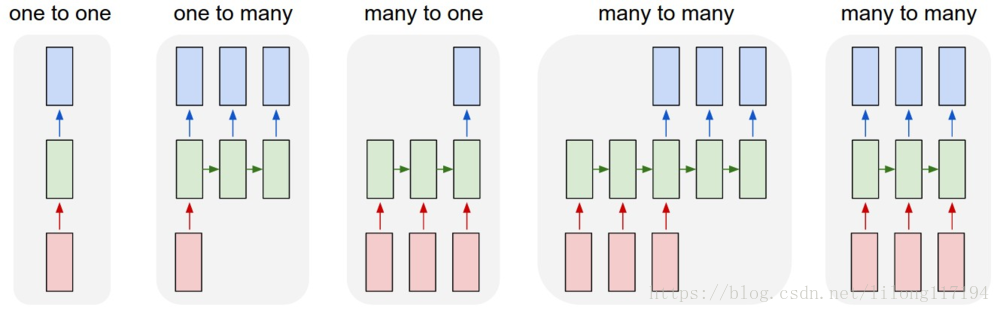
\includegraphics[width=\textwidth]{rnn_2}
\caption{RNN的多种模式}
\label{fig:rnn_2}
\end{figure}
%与常规的神经网络相比,循环神经网络以序列数据为输入,输出对应的序列数据结果。如图\ref{fig:rnn_2}所示,每一个矩形是一个向量,箭头则表示函数(如矩阵相乘)。输入向量用红色标出,输出向量用蓝色标出,绿色的矩形是RNN的状态。

1)单一输入和单一输出的Vanilla模型,例如图像分类任务;

2)单一输入序列输出,例如通过图片生成字幕;

3)序列输入单一输出,如自然语言情感分类任务,给定语句判断为积极或消极标签;

4)序列输入和序列输出,例如机器翻译任务;

5)同步输入输出,如视频分类任务。



%。其前向传播计算公式如下:
%\begin{align*}
%    r_t &= \sigma(W_r \cdot [h_{t-1},x_t]) \\
%    z_t &= \sigma(W_z \cdot [h_{t-1},x_t]) \\
%    \tilde{h_t} &= \tanh(W_{\tilde{h_t}}) \cdot [r_t \odot h_{t-1},x_t]) \\
%    h_t &= (1-z_t) \odot h_{t-1} +z_t \odot \tilde{h_t} \\
%    y_t &= \sigma(W_o \cdot h_t)
%\end{align*}
%其中方括号表示两个向量连接,$\odot$表示矩阵逐点相乘。
%

\subsection{本章小结}
本章第一节明确了分层存储的定义,并对当前主流的4层存储模型进行了阐述。与4层存储模型相对应的是数据的分类方式,主要包括I/O密集型、任务关联型、重要与敏感数据、归档数据等。在此存储模型下,数据分类的指标可归结为I/O性能要求、任务关联性以及外部环境要求等三方面。我们的研究针对任务关联性指标展开,为了捕捉文件之间的静态关联和较长时间跨度的任务关联性,本文建立了词嵌入模型和基于循环神经网络的模型,将在后续章节中逐一介绍。

第二节对自然语言处理领域的两个重要内容进行了介绍,一是词嵌入技术的发展概况和基本原理,尤其是近年来广泛应用的Word2Vec模型。二是介绍了循环神经网络的基本概况,阐明其在自然语言处理和序列处理中的广泛应用。随后阐述了LSTM神经网络基本原理及其解决长期依赖问题的特性。